
% ----------------------------------------------------------------------
%                   LATEX TEMPLATE FOR PhD THESIS
% ----------------------------------------------------------------------

% based on Harish Bhanderi's PhD/MPhil template, then Uni Cambridge
% http://www-h.eng.cam.ac.uk/help/tpl/textprocessing/ThesisStyle/
% corrected and extended in 2007 by Jakob Suckale, then MPI-CBG PhD programme
% and made available through OpenWetWare.org - the free biology wiki


%: Style file for Latex
% Most style definitions are in the external file PhDthesisPSnPDF.
% In this template package, it can be found in ./Latex/Classes/
\documentclass[oneside,12pt]{Latex/Classes/PhDthesisPSnPDF}
\usepackage{acro}

%: Macro file for Latex
% Macros help you summarise frequently repeated Latex commands.
% Here, they are placed in an external file /Latex/Macros/MacroFile1.tex
% An macro that you may use frequently is the figuremacro (see introduction.tex)
\include{Latex/Macros/MacroFile1}
\usepackage{nicefrac}
\usepackage{geometry}
\usepackage[sc]{mathpazo}
\usepackage{multirow}
\usepackage{float}
\usepackage{natbib}
\usepackage{listings}
\usepackage{appendix}
\usepackage{color,xcolor,soul}
\usepackage{enumitem}
\usepackage[titles]{tocloft} % remove dots from TOC
\renewcommand{\cftdot}{}
\usepackage{titlesec}

\titlespacing\section{0pt}{12pt plus 4pt minus 2pt}{0pt plus 2pt minus 2pt}
\titlespacing\subsection{0pt}{12pt plus 4pt minus 2pt}{0pt plus 2pt minus 2pt}
\titlespacing\subsubsection{0pt}{12pt plus 4pt minus 2pt}{0pt plus 2pt minus 2pt}

\makeatletter
\patchcmd{\@chapter}{\protect {CHAPTER }}{\ifappendix{APPENDIX }\else{CHAPTER }\fi}{}{}
\makeatother
\AtBeginEnvironment{appendices}{\appendixtrue}

\makeatletter
\setlength{\@fptop}{0pt}
\makeatother

\usepackage{titletoc}% http://ctan.org/pkg/titletoc % Appends CHAPTER 3 in TOC Chater names, UMaT standard
\titlecontents{chapter}% <section-type>
[0pt]% <left>
{}% <above-code>
{\MakeUppercase{\bfseries\chaptername}\ \bfseries\thecontentslabel\quad}% <numbered-entry-format>
{}% <numberless-entry-format>
{\bfseries\hfill\contentspage}% <filler-page-format>

\tolerance=1
\emergencystretch=\maxdimen
\hyphenpenalty=10000
\hbadness=10000

\setcitestyle{authoryear, round, longnamesfirst} % for harvard style 
%----------------------------------------------------------------------------------------
%	MARGIN SETTINGS // UMaT Thesis Guide
%----------------------------------------------------------------------------------------

\geometry{
	paper=a4paper, % Change to letterpaper for US letter
	inner=0.0cm, % Inner margin
	outer=0.0cm, % Outer margin
	%bindingoffset=.5cm, % Binding offset
	top=2.54cm, % Top margin
	bottom=2.54cm, % Bottom margin
	right=2.54cm, % Right margin
	left=3.02cm % Left margin, to allow space for binding UMaT, Tarkwa
	%showframe, % Uncomment to show how the type block is set on the page
}

%: ----------------------------------------------------------------------
%:                  TITLE PAGE: name, degree,..
% ----------------------------------------------------------------------
% below is to generate the title page with crest and author name

%if output to PDF then put the following in PDF header
\ifpdf  
    \pdfinfo { /Title  (PhD and MPhil Thesis Classes)
               /Creator (TeX)
               /Producer (pdfTeX)
               /Author (YourName your@email.net)
               /CreationDate (D:YYYYMMDDhhmmss)  %format D:YYYYMMDDhhmmss
               /ModDate (D:YYYYMMDDhhmm)
               /Subject (xyz)
               /Keywords (add, your, keywords, here) }
    \pdfcatalog { /PageMode (/UseOutlines)
                  /OpenAction (fitbh)  }
\fi


\title{DEVELOPMENT OF AN EFFICIENT PUBLIC TRANSPORT SEARCH PORTAL FOR GHANA}



% ----------------------------------------------------------------------
% The section below defines www links/email for author and institutions
% They will appear on the title page of the PDF and can be clicked
\ifpdf
  %\author{\href{mailto:your@email.net}{Your Name}}
  \author{{ENOCK SETH NYAMADOR}}
%  \cityofbirth{born in XYZ} % uncomment this if your university requires this
%  % If city of birth is required, also uncomment 2 sections in PhDthesisPSnPDF
%  % Just search for the "city" and you'll find them.
%  \collegeordept{\href{http://www.something.net}{CollegeOrDepartment}}
 \collegeordept{{DEPARTMENT OF COMPUTER SCIENCE AND ENGINEERING}}
%  \university{\href{http://www.something.net}{University}}
\university{{UNIVERSITY OF MINES AND TECHNOLOGY}}
  % The crest is a graphics file of the logo of your research institution.
  % Place it in ./0_frontmatter/figures and specify the width
  \crest{\includegraphics[width=4cm]{umatlogo}}
  
% If you are not creating a PDF then use the following. The default is PDF.
\else
  \author{ENOCK SETH NYAMADOR}
%  \cityofbirth{born in XYZ}
  \collegeordept{CollegeOrDept}
  \university{University}
  \crest{\includegraphics[width=4cm]{logo}}
\fi

%\renewcommand{\submittedtext}{change the default text here if needed}
\degree{BACHELOR OF SCIENCE}
\degreedate{MAY 2018}


% ----------------------------------------------------------------------
       
% turn of those nasty overfull and underfull hboxes
\hbadness=10000
\hfuzz=50pt

\setlength{\parindent}{0em}
\setlength{\parskip}{0.8em}


%: --------------------------------------------------------------
%:                  FRONT MATTER: dedications, abstract,..
% --------------------------------------------------------------

\begin{document}

%\language{english}

% sets line spacing
\renewcommand\baselinestretch{1.5}
\baselineskip=18pt plus1pt




%: ----------------------- generate cover page ------------------------

\maketitle  % command to print the title page with above variables


%: ----------------------- cover page back side ------------------------
% Your research institution may require reviewer names, etc.
% This cover back side is required by Dresden Med Fac; uncomment if needed.

\frontmatter
%: ----------------------- abstract ------------------------

% Your institution may have specific regulations if you need an abstract and where it is to be placed in the document. The default here is just after title.

% Thesis statement of originality -------------------------------------

% Depending on the regulations of your faculty you may need a declaration like the one below. This specific one is from the medical faculty of the university of Dresden.

\begin{declaration}        %this creates the heading for the declaration page



\end{declaration}


% ----------------------------------------------------------------------


% Thesis Abstract -----------------------------------------------------

%\begin{abstractslong}    %uncommenting this line, gives a different abstract heading
\begin{abstracts}        %this creates the heading for the abstract page
\addcontentsline{toc}{chapter}{ABSTRACT}
Public transport by road is the major means of transportation in Ghana. Information about operators, routes operated, departure times, location, etc are not readily available to the public outside the stations. This project seeks to make it easier for travelers to find information on transport routes and terminals in Ghana, enabling effective trip planning and decision making. A public transport search web portal application was developed to make access to route information easier for travelers. The application was developed using data collected and mapped into OpenStreetMap database. The data was extracted, cleaned and analysed in QGIS.  A geodatabase  was created using PostgreSQL and PostGIS to suit the needs of this project. The geodatabase can also be accessed by other stakeholders externally without interacting with the web application.
\end{abstracts}
%\end{abstractlongs}


% ---------------------------------------------------------------------- 


% The original template provides and abstractseparate environment, if your institution requires them to be separate. I think it's easier to print the abstract from the complete thesis by restricting printing to the relevant page.
% \begin{abstractseparate}
%   
% Thesis Abstract -----------------------------------------------------

%\begin{abstractslong}    %uncommenting this line, gives a different abstract heading
\begin{abstracts}        %this creates the heading for the abstract page
\addcontentsline{toc}{chapter}{ABSTRACT}
Public transport by road is the major means of transportation in Ghana. Information about operators, routes operated, departure times, location, etc are not readily available to the public outside the stations. This project seeks to make it easier for travelers to find information on transport routes and terminals in Ghana, enabling effective trip planning and decision making. A public transport search web portal application was developed to make access to route information easier for travelers. The application was developed using data collected and mapped into OpenStreetMap database. The data was extracted, cleaned and analysed in QGIS.  A geodatabase  was created using PostgreSQL and PostGIS to suit the needs of this project. The geodatabase can also be accessed by other stakeholders externally without interacting with the web application.
\end{abstracts}
%\end{abstractlongs}


% ---------------------------------------------------------------------- 

% \end{abstractseparate}


%: ----------------------- tie in front matter ------------------------


% Thesis Dedictation ---------------------------------------------------

\begin{dedication} %this creates the heading for the dedication page
This project wok is dedicated to my mother, Jamila Adams, Prince Ahiabu and Okatachie Afrifa Amankwaa. Your unending love and supports is highly appreciated.  

\end{dedication}

% ----------------------------------------------------------------------

% Thesis Acknowledgements ------------------------------------------------


%\begin{acknowledgementslong} %uncommenting this line, gives a different acknowledgements heading
\begin{acknowledgements}      %this creates the heading for the acknowlegments
\addcontentsline{toc}{chapter}{\textbf{ACKNOWLEDGEMENTS}}
I am grateful to Dr Hamidu Abdel-Fatao, my project supervisor for guiding me through the writing of this report, and my lecturers who equipped me with the knowledge required to write it.
\end{acknowledgements}
%\end{acknowledgmentslong}

% ------------------------------------------------------------------------




%: ----------------------- contents ------------------------

\setcounter{secnumdepth}{3} % organisational level that receives a numbers
\setcounter{tocdepth}{3}    % print table of contents for level 3
\renewcommand\contentsname{TABLE OF CONTENTS}
\tableofcontents            % print the table of contents
% levels are: 0 - chapter, 1 - section, 2 - subsection, 3 - subsection


%: ----------------------- list of figures/tables ------------------------
\renewcommand\listfigurename{\textbf{LIST OF FIGURES}}
\listoffigures	% print list of figures

%\listoftables  % print list of tables


%: ----------------------- glossary ------------------------

% Tie in external source file for definitions: /0_frontmatter/glossary.tex
% Glossary entries can also be defined in the main text. See glossary.tex
%\include{0_frontmatter/glossary} 

%\begin{multicols}{2} % \begin{multicols}{#columns}[header text][space]
%\begin{footnotesize} % scriptsize(7) < footnotesize(8) < small (9) < normal (10)

%\printnomenclature[1.5cm] % [] = distance between entry and description
%\label{nom} % target name for links to glossary
%
%\end{footnotesize}
%\end{multicols}



%: --------------------------------------------------------------
%:                  MAIN DOCUMENT SECTION
% --------------------------------------------------------------

% the main text starts here with the introduction, 1st chapter,...
\mainmatter

%\renewcommand{\chaptername}{} % uncomment to print only "1" not "Chapter 1"


%: ----------------------- subdocuments ------------------------

% Parts of the thesis are included below. Rename the files as required.
% But take care that the paths match. You can also change the order of appearance by moving the include commands.


% this file is called up by thesis.tex
% content in this file will be fed into the main document

%: ----------------------- introduction file header -----------------------
\chapter{Introduction}

% the code below specifies where the figures are stored
\ifpdf
    \graphicspath{{1_introduction/figures/PNG/}{1_introduction/figures/PDF/}{1_introduction/figures/}}
\else
    \graphicspath{{1_introduction/figures/EPS/}{1_introduction/figures/}}
\fi

% ----------------------------------------------------------------------
%: ----------------------- introduction content ----------------------- 
% ----------------------------------------------------------------------



%: ----------------------- HELP: latex document organisation
% the commands below help you to subdivide and organise your thesis
%    \chapter{}       = level 1, top level
%    \section{}       = level 2
%    \subsection{}    = level 3
%    \subsubsection{} = level 4
% note that everything after the percentage sign is hidden from output

\section{Problem Statement}
Road transport service provided by both formal and informal sectors in Ghana is by far the most popular and principal means of conveying passengers, goods and other services between any two or more locations \citep{aidoo_passengers_2013}. Some report have it that, road transport carries over $ 95\% $ of all passenger and freight traffic and about $ 97\% $ of all passenger miles in Ghana \citep[p.~195]{unesco_transportation:_????}, a country that is experiencing rapid demographic and economic growth. The vast majority of passengers commuting between places, be it \textit{intra-city} or \textit{inter-city}, mostly rely on public transport services in the form of privately owned or corporate taxis, \textit{tro tros} (shared minivans), buses commuting between major cities.

In spite of the heavy reliance on public road transport services by the general populace in Ghana, finding transport terminals which offer reliable road transport services is not as easy as it should be. The difficulty in finding transport terminals is attributable to the fact that little or no information about the availability of transport services and their locations is accessible to the public. Additionally, the non-existent of a means to compare transport fares by various service providers often makes it difficult for the potential passenger to make the right choices. It is the goal of every potential passenger to find the fastest, safest and most cost-efficient means of transiting from one location to another. 

Inspired by the aforementioned shortcomings of the existing public road transportation system, this project seeks to develop road transport terminal search tool
aimed at mitigating, if not eliminate entirely, these problems with the public road transport industry.

\newpage
\section{Project Objectives}
The objective of this project include the following:
\begin{itemize}
	\item To develop a web application that provides detailed information about transport terminals in Ghana to mitigate the difficulty in finding transport terminals and also to provide a platform for to compare other factors by travelers.
	%	\item To provide \hl{reusable data} that can be accessed in mobile and desktop applications that support Geo Uniform Resource Identifier (URI) scheme.
	%	\item With Global Positioning System (GPS) supported devices, the work also provides a means of navigating to destination based by incorporating existing mapping solution such as
	%    \begin{itemize}[label=$\circ$]
	%	\item OSMAnd
	%	\item MAPS.ME
	%	\item Google Maps
	%	\item Apple Maps
	%	\item Marble
	%	\item Google Earth
	%	\end{itemize}
\end{itemize}

\section{Project Outcomes}
The following will be achieved at the end of the project:
\begin{itemize}
	\item An web application;
%	\item \sout{Possibly generate high definition printer friendly maps that serves nearly same purpose as the web platform.}
	\item A detail map of selected transport terminals on OpenStreetMap.
\end{itemize}


\section{Methods used}
The methods to be used for the project are as below:
\begin{itemize}
	\item Literature review on proposed topic
	\item Study and understanding of online maps (creating, updating, deleting);
	\item The system will be developed on a handful of local machines, but with scalability and ease of deployment on any kind of infrastructure;
	\item The system will be prototyped in Python programming language and Django web framework. If this language proves good enough for deployment purposes it will be used in the final product;
	\item Survey and crowd-sourcing information on some transport terminals to facilitate database creation;
	\item QGIS will be used to clean and analyze data collected;
	\item Spiral software development model.
\end{itemize}

\section{Tools and Facilities used}
The facilities required for this project include:
\begin{itemize}
	\item University of Mines and Technology (UMaT) library;
	\item Internet;
	\item General search engines as such Wikipedia and DuckDuckGo;
	\item Open Source software repositories such as GitHub;
	\item OpenStreetMap;
	\item Documentation of any software or libraries used.
\end{itemize}

\section{Scope of Work}
This works seeks to aid travelers acquire detailed information on selected bus terminals in Ghana. This is to enable better trip planning, reduce time taken finding these terminals and also allowing passengers to compare transport fares and choosing the best option they can afford.
Further more the application only indicates source and destination terminals and works in the any modern web browser such as Mozilla Firefox or Google Chrome.

\section{Organization of Project}
This project is divided into five chapters. The first chapter talks about the problem to be solved, the objectives, the methods, tools and facilities used, and project outcomes. The second chapter discusses relevant literature and related works. The third chapter discusses how the problem was solved. The fourth chapter talks about the operation of the developed application. The project concludes in the fifth chapter where, limitations and recommendations for future improvements were discussed.

	% background information
% this file is called up by thesis.tex
% content in this file will be fed into the main document

\chapter{Introduction} % top level followed by section, subsection


% ----------------------- contents from here ------------------------

\section{}

\subsection{}
\subsubsection{}




% ---------------------------------------------------------------------------
% ----------------------- end of thesis sub-document ------------------------
% ---------------------------------------------------------------------------
						% aims of the project
% this file is called up by thesis.tex
% content in this file will be fed into the main document

%: ----------------------- name of chapter  -------------------------
\chapter{Software Design and Analysis} % top level followed by section, subsection


%: ----------------------- paths to graphics ------------------------

% change according to folder and file names
\ifpdf
    \graphicspath{{3/figures/PNG/}{3/figures/PDF/}{3/figures/}}
\else
    \graphicspath{{3/figures/EPS/}{3/figures/}}
\fi

%: ----------------------- contents from here ------------------------
\section{Overview}
In this chapter, the software (Public Transportation Search Web Portal) development life cycle has been discussed.

\section{Software Development Process Model}
A software development process model is simply the process by which an organization 
develops software. (Zeil, 2016). It is broken down into several phases, there are different criteria for each phase \citep{marciniak1994encyclopedia}. The software development model chosen here is the spiral model. This model was chosen due to the exploratory nature of the project.

The spiral model cycles through four quadrants, each representing a particular development phase \cite{boehm_spiral_1988}. The cycle is shown in Figure 3.1.

\begin{figure}[th!]
	\centering
	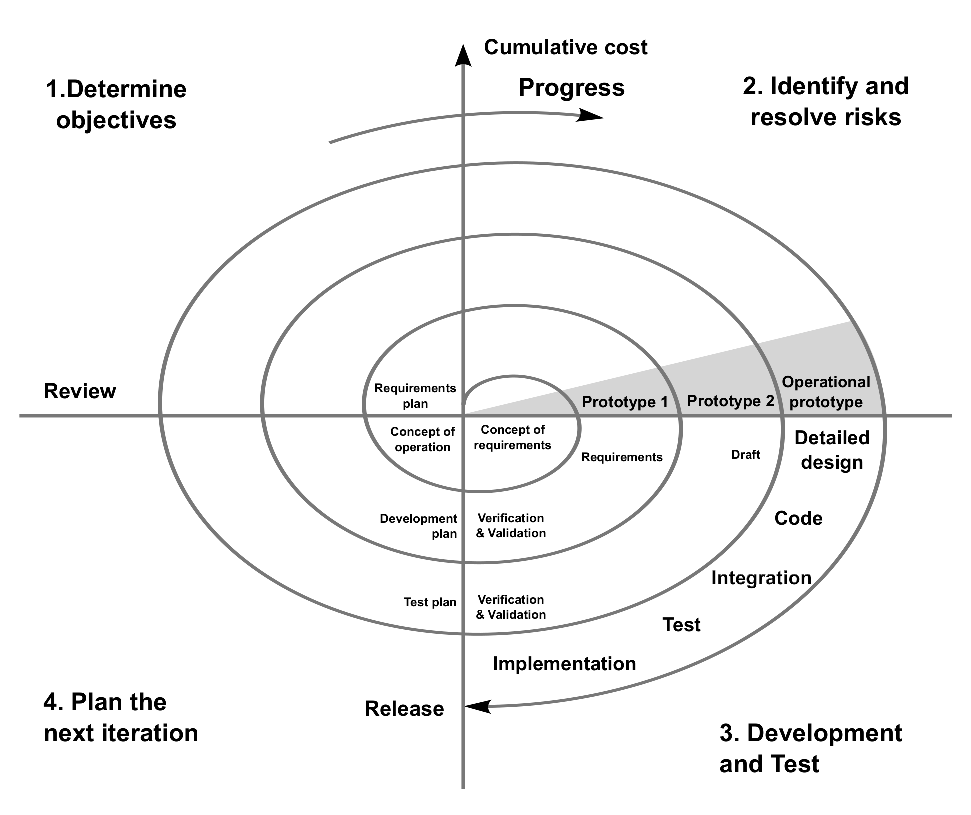
\includegraphics[width=0.7\textwidth]{spiral}
	\caption[The Spiral Model of Software Development]{The Spiral Model of Software Development}
	\label{fig:spiral}
\end{figure}

\subsection{Phases of the Spiral Model}
The phases of the spiral model includes:

\subsubsection{Determine Objectives, Alternatives and Constraints}
During this phase the objectives for the iteration, and it's alternatives and constraints are investigated.

\subsubsection{Evaluate Alternatives, Identify and Resolve Risks}
The risks involved in the iteration of development are examined, and solutions are found. Additionally, this phase also evaluates the alternatives to the chosen strategy.

\subsubsection{Develop and Verify the Next Level Product}
The development of the product takes place in this phase. For each cycle a different methodology may be used during this phase. For instance, the waterfall model can be used for 

\subsubsection{Plan Next Iteration}
During this phase, with all the information gained from the past cycles, the next iteration is planned.

\subsection{Advantages of the Spiral Model}
The advantages of the Spiral Model are as follows:
\begin{itemize}
	\item It enhances risk avoidance;
	\item A different methodology can be selected for each iteration; and 
	\item It can incorporate the Waterfall, Prototype and Incremental methodologies.
\end{itemize}

\section{Feasibility Studies and Analyses}
Feasibility studies are some preliminary studies undertaken to know whether the project is feasible or not, given a number of circumstances. These studies include; technical, time frame, availability of funds, legal and ethical issues, availability of funds and resources, operation and marketing.

\section{Requirements Gathering}
A number of questions were asked and answers determined from stakeholders and other interest groups during requirements gathering. Some these questions include:
		\begin{itemize}		
			\item Where is the system going to be used? (Ghana)
			\item Who is going to use the system? (Traveler)
			\item What data should be input into the system? (Text)
			\item What Software Development Life Cycle (SDLC) model to be used? (Spiral)
			\item What type of output information will the system give? (Text and map data)
		\end{itemize}

\subsection{Cost Analysis}
Since this is a software only project we will not concern ourselves with price of hardware.  However, the price of the hardware is directly to the resources used, which were analysed in the feasibility study. Therefore it is concluded hat this system will depend on the size of data being added to the database and traffic to application.

\subsection{Risk Analysis}
The two main risks involved in this project are the security risks anyone hosting services on the internet will face, and the risk of invalid data or information added by staff or administrator to the database.\\

The first risk is mitigated by limiting the surface area of the system exposed to attackers and by strengthening the components which have been exposed. In this system, the only such component is the search front-end. The search front-end only has read access to the database. Since the information stored therein is public, the only thing a malicious actor can do with this is cause a Denial-of-Service (DoS) attack. Appropriate steps will be taken to mitigate this.\\

The second risk somewhat complex to identify in some cases. Data will pass through several stages of validation and clean up before being made available to the public in order to provide them with the right information.

\subsection{Use Case Diagram}
A Use Case diagram depicts how the users interact with the system. It describes which operations the system can perform and the users as shown in Figure \ref{fig:usecase} below.

\begin{figure}[H]
	\centering
	\includegraphics[width=0.9\linewidth]{usecase}
	\caption[Use Case Diangram]{Use Case Diangram}
	\label{fig:usecase}
\end{figure}


\subsection{Activity Diagram}
An activity diagram visually presents a series of actions or flow of control in a system similar to a flowchart or or data flow diagram 

An activity refers to a particular operation of a system. The operations in this system are modeled in to the the activity diagram in Figure \ref{fig:activitydiagram} below.

\begin{figure}[H]
	\centering
	\includegraphics[width=0.5\linewidth]{activitydiagram}
	\caption[Activity Diagram]{Activity Diagram}
	\label{fig:activitydiagram}
\end{figure}


\section{Implementation}
The application is set into operation at the implementation stage. This includes how data is taken by the system, what form of data is taken by the system, where the data is kept, how the data is processed and what form of information is outputted. The first step was to collect and map out transport terminals detailed information in some parts of Ghana; including but no limited to:
\begin{itemize}
	\item Name
	\item Location (\textit{Town name})
	\item Location (\textit{Longitude and Latitude})
	\item Contacts (\textit{Phone, Email, Website, Operator})
	\item Operators (\textit{STC, GRPTU, VVIP, VIP})
	\item Destinations
	\item Departure times
	\item Vehicle types
\end{itemize}

The mapped data was uploaded to OpenStreetMap database. After the mapping of the lorry stations, the mapped data was extracted and processed in QGIS before being imported into the projects local PostgreSQL based database.

\begin{figure}[H]
	\centering
	\includegraphics[width=0.7\linewidth]{3/figures/overpass}
	\caption[Extracting mapped data from OpenStreetMap]{Extracting mapped data from OpenStreetMap}
	\label{fig:overpass}
\end{figure}


\subsection{Data Collection}
Data was collected using smartphones and handheld GPS receivers. The following information were collected from the selected lorry stations. Some of these information was collected by survey and crowdsouring tickets. Some of the data recorded include:
\begin{itemize}
	\item Name;
	\item Operator;
	\item Departure time;
	\item Fares; and 
	\item Available destinations.
\end{itemize}

\begin{figure}[H]
	\centering
	\includegraphics[width=0.6\linewidth]{ticket}
	\caption[Sample bus ticket]{Sample bus ticket}
	\label{fig:ticket}
\end{figure}

\begin{figure}[H]
	\centering
	\includegraphics[width=0.6\linewidth]{schedules}
	\caption[Information available within terminals]{Information available within terminals}
	\label{fig:schedules}
\end{figure}

\subsection{Mapping Transportation Terminals}
The following steps were taken in the mapping out process:
\begin{itemize}
	\item Go to \textit{https://www.osm.org} in a modern web browser such as Firefox of Chromium; 
	\item Searched for town or city where lorry station is to be mapped; and 
	\item Area was edited by using JOSM editor as shown in Figure \ref{fig:josm};
	\item Marking out specific areas (buildings, routes (roads, walkways) and the stations are either mapped as points or closed ways (polygons);  
	\item Naming  and describing of point, areas or routes. 
\end{itemize}

\begin{figure}[H]
	\centering
	\includegraphics[width=0.8\linewidth]{josm}
	\caption[Mapping Bus Station into OpenStreetMap]{Mapping Bus Station into OpenStreetMap}
	\label{fig:josm}
\end{figure}

\subsection{Rendering of maps and Routing}
The map showing location various stations was rendered using Leaflet. Routing is from departure station is done on the web using the Open Source Routing Machine (OSMRM) Car and OpenStreetMap as a basemap. When the routes and stations locations are accessed from a smartphone with any map application such as OSMAnd, MAPS.ME, Google Maps, etc they will be prompted to choose and option or else it is opened in a web browser.


% ---------------------------------------------------------------------------
%: ----------------------- end of thesis sub-document ------------------------
% ---------------------------------------------------------------------------

						% system design and analysis
% this file is called up by thesis.tex
% content in this file will be fed into the main document

%: ----------------------- name of chapter  -------------------------
\chapter{System Operation} % top level followed by section, subsection


%: ----------------------- paths to graphics ------------------------

% change according to folder and file names
\ifpdf
    \graphicspath{{4/figures/PNG/}{4/figures/PDF/}{4/figures/}}
\else
    \graphicspath{{4/figures/EPS/}{4/figures/}}
\fi

%: ----------------------- contents from here ------------------------
\section{Overview}
This shows how the system works after its implementation. 

\section{System Operation}
When the application is started as shown in Figure 4.1 below. Users are prompted to enter both their \textit{departure} and \textit{destination} towns or cities.


\section{Back End}
Administration
User login
Add stations
Add Operators
Add routes
Ad users

\section{Front End}
Homepage
User search destination and departure
Results
Route details
\begin{figure}[H]
	\centering
	\includegraphics[width=1\linewidth]{routeinfo}
	\caption[Route Information]{Route Information}
	\label{fig:routeinfo}
\end{figure}

-- View Routing on map
View station detail






% ---------------------------------------------------------------------------
%: ----------------------- end of thesis sub-document ------------------------
% ---------------------------------------------------------------------------


% this file is called up by thesis.tex
% content in this file will be fed into the main document

%: ----------------------- name of chapter  -------------------------
\chapter{Conclusions and Recommendations} % top level followed by section, subsection


%: ----------------------- paths to graphics ------------------------

% change according to folder and file names
\ifpdf
    \graphicspath{{5/figures/PNG/}{5/figures/PDF/}{5/figures/}}
\else
    \graphicspath{{5/figures/EPS/}{5/figures/}}
\fi

%: ----------------------- contents from here ------------------------
\section{Conclusion}
In this project, a web application was developed to help travelers find detail information whcih always available on arrival at the various terminals and stations but not readily available to them prior to starting to their journey. To accomplish this project, some terminals and stations were clearly mapped on OpenStreetMap. After mapping, the data was extracted and further processed to create a geodatabase using PostgreSQL and PostGIS. The data was rendered with Leaflet. Search and routing functionality were subsequently added. The developed application has map rendering and text based interaction to input and output features. It can therefore be concluded that the application will improve trip planning and easy access to information only available within terminals to travelers hence saving time and other resources.It could also be adopted by Ghana Tourism Authority to help tourists find their way around Ghana transport network.

The future objective is to deploy the application making it available for public use in Ghana.

\section{Recommendations}
This project recommends that users should be able to book seats from the platform and also support voice input for the visually impaired as well. The system should get users current location and find nearest available departure stations for their routes. Also a commenting system for users to interact and share experiences about each route.

% ---------------------------------------------------------------------------
%: ----------------------- end of thesis sub-document ------------------------
% ---------------------------------------------------------------------------



% --------------------------------------------------------------
%:                  BACK MATTER: appendices, refs,..
% --------------------------------------------------------------

% the back matter: appendix and references close the thesis


%: ----------------------- bibliography ------------------------

% The section below defines how references are listed and formatted
% The default below is 2 columns, small font, complete author names.
% Entries are also linked back to the page number in the text and to external URL if provided in the BibTex file.

% PhDbiblio-url2 = names small caps, title bold & hyperlinked, link to page 
%\begin{multicols}{2} % \begin{multicols}{ # columns}[ header text][ space]
%\begin{tiny} % tiny(5) < scriptsize(7) < footnotesize(8) < small (9)

\bibliographystyle{Latex/Classes/agsm-umat} % Title is link if provided
\renewcommand{\bibname}{\textbf{REFERENCES}} % changes the header; default: Bibliography

\bibliography{9_backmatter/references} % adjust this to fit your BibTex file

%\end{tiny}
%\end{multicols}

% --------------------------------------------------------------
% Various bibliography styles exit. Replace above style as desired.

% in-text refs: (1) (1; 2)
% ref list: alphabetical; author(s) in small caps; initials last name; page(s)
%\bibliographystyle{Latex/Classes/PhDbiblio-case} % title forced lower case
%\bibliographystyle{Latex/Classes/PhDbiblio-bold} % title as in bibtex but bold
%\bibliographystyle{Latex/Classes/PhDbiblio-url} % bold + www link if provided

%\bibliographystyle{Latex/Classes/jmb} % calls style file jmb.bst
% in-text refs: author (year) without brackets
% ref list: alphabetical; author(s) in normal font; last name, initials; page(s)

%\bibliographystyle{plainnat} % calls style file plainnat.bst
% in-text refs: author (year) without brackets
% (this works with package natbib)


% --------------------------------------------------------------

% according to Dresden med fac summary has to be at the end
%
% Thesis Abstract -----------------------------------------------------

%\begin{abstractslong}    %uncommenting this line, gives a different abstract heading
\begin{abstracts}        %this creates the heading for the abstract page
\addcontentsline{toc}{chapter}{ABSTRACT}
Public transport by road is the major means of transportation in Ghana. Information about operators, routes operated, departure times, location, etc are not readily available to the public outside the stations. This project seeks to make it easier for travelers to find information on transport routes and terminals in Ghana, enabling effective trip planning and decision making. A public transport search web portal application was developed to make access to route information easier for travelers. The application was developed using data collected and mapped into OpenStreetMap database. The data was extracted, cleaned and analysed in QGIS.  A geodatabase  was created using PostgreSQL and PostGIS to suit the needs of this project. The geodatabase can also be accessed by other stakeholders externally without interacting with the web application.
\end{abstracts}
%\end{abstractlongs}


% ---------------------------------------------------------------------- 


%: Declaration of originality
\appendix
\addtocontents{toc}{\protect\renewcommand\protect\chaptername{Appendix}}
%\renewcommand\chaptername{Appendix}
\chapter{A SAMPLE CODE FOR MODELS } 
\lstinputlisting[language=Python]{/home/kakarot/terminalfinder/terminal/models.py}
\end{document}
